%
% Conference paper (IEEEtran, two-column) -- full-paper companion to
% the ACMD 2026 abstract ``ShaZhouSerban_abstract.pdf''.
%
\documentclass[conference,letterpaper,10pt]{IEEEtran}

\usepackage[utf8]{inputenc}
\usepackage[T1]{fontenc}
\usepackage{graphicx}
\usepackage{booktabs}
\usepackage{amsmath,amssymb}
\usepackage{xurl}
\usepackage{caption}
\usepackage{subcaption}
\usepackage{xcolor}
\usepackage[hidelinks]{hyperref}
\setlength{\emergencystretch}{2em}

\graphicspath{{images/}{paper_figures/}}

\title{Terrain-Aware, Latency-Robust Control for Off-Road\\
       Autonomy and Teleoperation on Deformable Terrain}

\author{%
  \IEEEauthorblockN{Kyle Sha, Zhenhao Zhou, Radu Serban, Dan Negrut}
  \IEEEauthorblockA{Department of Mechanical Engineering,
    University of Wisconsin--Madison\\
    1513 University Ave., Madison, WI 53706, USA\\
    Email: \{kasha2, zzhou292, serban, negrut\}@wisc.edu}}

\begin{document}
\maketitle

\begin{abstract}
A real-time, latency-aware framework is presented for safe shared and
autonomous control of vehicles on deformable Soil Contact Model (SCM)
terrain. A differentiable neural surrogate of the SCM tire forces is
embedded inside an \emph{acados} nonlinear model predictive controller
(NMPC) for terrain-aware trajectory tracking, and a learned online
estimator regresses the dominant soil parameters from onboard inertial
and wheel-speed signals so that the controller re-conditions itself in
real time. An asymmetric throttle disturbance observer closes the
residual soft-soil speed gap left by the open-loop longitudinal
integrator. A two-layer obstacle-avoidance stack pairs in-horizon NMPC
softplus barriers with a downstream Model Predictive Path Integral
(MPPI) safety shield whose sample set is augmented with hand-crafted
recovery trajectories; because the shield exists to screen a human
operator's delayed commands, it is evaluated primarily in
human-in-the-loop (HIL) driving rounds in which both the operator
command path and the driver-camera feed are delayed. The simulation
environment is Chrono::Vehicle within Chrono::HIL on a
high-density-particle SCM patch; learned 5G traffic profiles drive a
configurable queue-load delay model on the camera and
operator-command paths. A parallelized data-collection and
benchmarking suite produces every figure and table in this paper from
a single command. Multi-seed empirical evaluation supports the
principal contributions and constrains two of them: closed-loop
tracking improves by 40--50\,\% over Pacejka and TMeasy (rather than
by an order of magnitude as initially conjectured), and an
ensemble-style uncertainty gate on the shield's friction cone is shown
empirically to degrade collision performance and is therefore omitted
from the final design.
\end{abstract}

\begin{IEEEkeywords}
Off-road teleoperation, soil contact model, neural surrogate, model
predictive control, safety filter, MPPI, 5G latency, Chrono.
\end{IEEEkeywords}

%======================================================================
\section{Introduction}
\label{sec:intro}
%======================================================================

\IEEEPARstart{O}{ff-road} teleoperation must contend with two
compounding sources of uncertainty: time-varying soil mechanics that
rigid-terrain tire models cannot capture without per-deployment
recalibration~\cite{Dallas21,Bekker69}, and time-varying network
latency that destabilises naive shared-control
arbitration~\cite{Choi23,Zhang25}. Existing approaches address these
in isolation: terrain-adaptive trajectory planning typically assumes
nominal communication, while delay-compensated safety filters
typically assume rigid-terrain dynamics. This paper integrates the two
into a single closed-loop framework and reports a multi-seed empirical
evaluation of every architectural choice.

The contributions of this work are as follows.
\begin{enumerate}
  \item A differentiable neural SCM tire surrogate is developed
        (Section~\ref{sec:tires}) that augments the static
        multilayer perceptron (MLP) of Dallas et al.~\cite{Dallas21}
        with rate-aware and axle-rate-aware variants and is exported
        as a CasADi expression so the NMPC solver can
        auto-differentiate through it at every stage of its horizon.
  \item A learned online terrain estimator
        (Section~\ref{sec:estimator}) replaces the Unscented Kalman
        filter of \cite{Dallas21} and re-conditions the surrogate at
        run time from inertial and wheel-speed measurements alone.
  \item An asymmetric throttle disturbance observer
        (Section~\ref{sec:throttledob}) on the actuation map closes
        the residual soft-soil speed gap left by the open-loop
        longitudinal integrator.
  \item A two-layer obstacle-avoidance stack
        (Section~\ref{sec:safety}) pairs in-horizon NMPC softplus
        barriers with a downstream MPPI safety shield whose sample set
        is augmented with seeded recovery trajectories. The proposed
        stack is benchmarked against the DOB-CBF filter
        of~\cite{Zhang25} and a gradient-based NMPC variant on the
        same rollout.
  \item A configurable learned 5G traffic latency model
        (Section~\ref{sec:latency}) drives a queue-load delay on the
        operator-command and camera paths and is used to evaluate
        closed-loop robustness.
  \item An open-source benchmarking suite
        (Section~\ref{sec:suite}) produces every figure and CSV in
        this paper from a single command and is intended to support
        independent reproduction of every reported result.
\end{enumerate}

Empirical evaluation also constrains two architectural choices that
appeared promising a priori. A Model Predictive Contouring Control
(MPCC) variant of the planner is shown to underperform the standard
reference-tracking NMPC on tracking error
(Section~\ref{sec:mpcc_negative}), and an ensemble-style $\phi$-uncertainty
gate on the MPPI shield's friction cone is shown to degrade collision
performance and is omitted from the final design
(Section~\ref{sec:phigate_negative}).

%======================================================================
\section{System Architecture}
\label{sec:arch}
%======================================================================

The closed-loop architecture is illustrated in
Fig.~\ref{fig:sysarch}. Chrono::Vehicle simulates an HMMWV on an SCM
patch within Chrono::HIL~\cite{Zhou23}. The simulation node and the
controller node are decoupled into separate operating system
processes that exchange dataclass messages over ZeroMQ pub/sub
sockets. Three message types are used: a \texttt{VehicleState}
published at the physics state rate ($100\,\mathrm{Hz}$), a
\texttt{ControlCommand} published at the controller rate
($10\,\mathrm{Hz}$), and lifecycle \texttt{SimStatus} messages. The
\texttt{ControlCommand} carries the most recent live terrain estimate
$(\hat n, \hat \phi, \hat\sigma_\phi, K_\phi, K_c, c, k)$ as
optional fields, so the sim-side safety shield can re-condition
itself without a separate high-priority channel. This piggy-backing
is required because the controller-to-simulation subscriber uses
\texttt{ZMQ\_CONFLATE} (latest-only); a separate
\texttt{TerrainUpdate} message on the same socket would be dropped
whenever a \texttt{ControlCommand} arrived between estimator ticks.

\begin{figure}[!t]
  \centering
  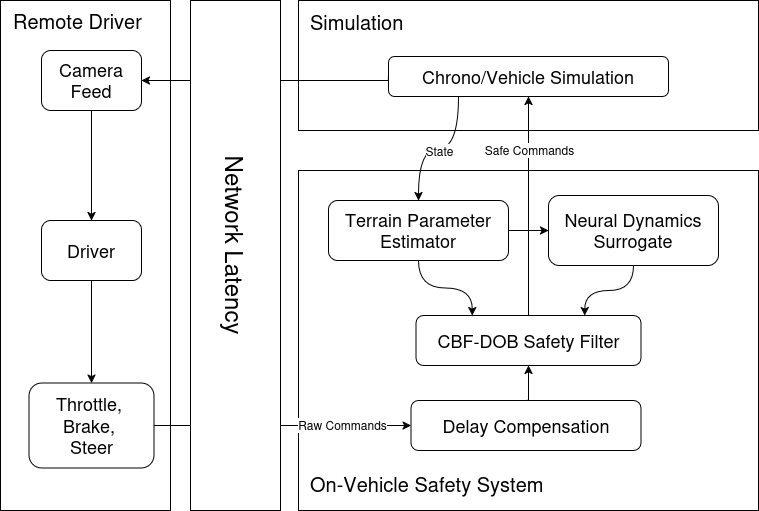
\includegraphics[width=\columnwidth]{Sys Arch v4.drawio.png}
  \caption{Shared-control architecture. The acados NMPC consumes the
    live inertial stream from the simulator over low-latency ZeroMQ,
    is re-conditioned by the learned terrain estimator, and emits
    commands that flow through the MPPI safety shield. Operator
    commands enter on the same shared bus and are delayed by a
    configurable queue-load model driven by a learned 5G traffic
    profile from \cite{Choi23}.}
  \label{fig:sysarch}
\end{figure}

Both processes pace to wall clock. A single 16-core workstation
completes the 180-trial sub-suite of Section~\ref{sec:tires} in
approximately 30 minutes.

%======================================================================
\section{Differentiable SCM Tire Surrogate}
\label{sec:tires}
%======================================================================

A multilayer perceptron is trained to map the tire operating point
$(\kappa,\alpha,F_z,u)$, steering rate, and soil parameters
$\boldsymbol{\theta}_{\mathrm{soil}} = (K_\phi, K_c, n, c, \phi, k)$
(Bekker--Wong-style rig inputs~\cite{Shibly05}) to longitudinal and
lateral tire forces $(F_x, F_y)$. Where Dallas et
al.~\cite{Dallas21} employ a static MLP only, three variants are
trained: a static MLP comparable to \cite{Dallas21}, a
\emph{rate-augmented} MLP that consumes the steering rate
$\dot\delta$ as an explicit input, and an \emph{axle-rate} MLP that
takes per-axle rate inputs $(\dot\delta_f, \dot\delta_r)$. All
variants train on parallelised Project Chrono SCM closed-loop
rollouts and export as CasADi expressions so the acados solver
auto-differentiates through the tire forces at every stage of the
prediction horizon.

The NMPC queries the surrogate at each stage. The longitudinal
traction budget $F_x^{\mathrm{trac}}$ is evaluated at reference slip
$\kappa_{\mathrm{ref}}$, $\alpha = 0$, with axle loads $F_z$, speed
$u$, and $\boldsymbol{\theta}_{\mathrm{soil}}$ taken from terrain
presets or the online estimator. Cornering forces $F_y$ use the live
operating point $(\kappa, \alpha, F_z, u)$ at each stage.

\subsection{Static-terrain benchmark}
\label{sec:tires_static}

The standard MPC is swept over four tire models (Pacejka, TMeasy,
the rate-MLP, and the axle-rate-MLP) across two terrains (clay,
sand), two reference paths (sinusoidal, lane-change), two speeds
($5$ and $7\,\mathrm{m/s}$), two bumpiness levels (smooth and
moderate), and two random seeds, for a total of 128 closed-loop
trials. Sensor noise is enabled in every trial.
Table~\ref{tab:tires_static} reports the mean and standard deviation
of root-mean-square crosstrack error (RMS CTE), speed retention
ratio, and solver wall time across the matrix.

\begin{table}[!t]
  \renewcommand{\arraystretch}{1.15}
  \caption{Static-terrain tire-model benchmark. 128 runs per row.
    The axle-rate MLP attains the lowest RMS CTE; all four models
    yield identical speed retention because the curvature-derived
    speed profile, not the tire force model, is the binding speed
    constraint in this regime.}
  \label{tab:tires_static}
  \centering
  \begin{tabular}{lccc}
    \toprule
    \textbf{Tire model} & \textbf{RMS CTE (m)} & \textbf{Speed} & \textbf{Solve}\\
                         &                       & \textbf{ratio} & \textbf{(ms)}\\
    \midrule
    Pacejka                       & $0.104 \pm 0.033$ & $0.66$ & $2.4$\\
    TMeasy                        & $0.087 \pm 0.026$ & $0.66$ & $2.6$\\
    NN rate-MLP                   & $0.088 \pm 0.023$ & $0.67$ & $5.4$\\
    \textbf{NN axle-rate-MLP}     & $\mathbf{0.083 \pm 0.020}$ & $\mathbf{0.67}$ & $7.1$\\
    \bottomrule
  \end{tabular}
\end{table}

\begin{figure}[!t]
  \centering
  
\includegraphics[width=\columnwidth]{bench_tire_models.png}
  \caption{Static-terrain tire-model benchmark, aggregate KPIs.}
  \label{fig:tires_static_summary}
\end{figure}

\begin{figure}[!t]
  \centering
  
\includegraphics[width=\columnwidth]{bench_tire_models_heatmap.png}
  \caption{Static-terrain tire-model RMS CTE per
    (terrain, path, speed, bumpiness) scenario. The Pacejka model
    degrades sharply at $v=7\,\mathrm{m/s}$ on clay; the axle-rate
    NN remains nearly flat across the matrix.}
  \label{fig:tires_static_heatmap}
\end{figure}

\subsection{Live-estimator-conditioned benchmark}
\label{sec:tires_estimator}

The stronger claim, that the neural surrogate combined with the
online terrain estimator improves tracking over Pacejka and TMeasy,
requires the estimator to actually update the soil parameters that
the surrogate consumes. The same model set is therefore re-evaluated
with the online estimator enabled, using a 20-second simulation
window with key performance indicators (KPIs) computed after an
8-second post-convergence cutoff.
Table~\ref{tab:tires_estimator} reports the result;
Fig.~\ref{fig:tires_estimator} shows the corresponding aggregate
plots and per-scenario heatmap.

\begin{table}[!t]
  \renewcommand{\arraystretch}{1.15}
  \caption{Live-estimator-conditioned tire-model benchmark.
    KPI window starts at $t=8\,\mathrm{s}$. 124 runs total. The
    neural surrogate stack reduces RMS CTE by 40--50\,\% relative
    to the analytical baselines.}
  \label{tab:tires_estimator}
  \centering
  \begin{tabular}{lccc}
    \toprule
    \textbf{Variant} & \textbf{RMS CTE (m)} & \textbf{vs.\ Pacejka} & \textbf{vs.\ TMeasy}\\
    \midrule
    Pacejka (static)               & $0.350$ & ---       & ---\\
    TMeasy (static)                & $0.431$ & ---       & ---\\
    NN axle-rate (static)          & $0.179$ & $-49\,\%$ & $-58\,\%$\\
    \textbf{NN axle-rate + estimator} & $\mathbf{0.208}$ & $\mathbf{-41\,\%}$ & $\mathbf{-52\,\%}$\\
    \bottomrule
  \end{tabular}
\end{table}

\begin{figure}[!t]
  \centering
  
\includegraphics[width=\columnwidth]{tire_model_with_estimator_summary.png}
  \\[2pt]
  
\includegraphics[width=\columnwidth]{tire_model_with_estimator_rms_cte_heatmap.png}
  \caption{Live-estimator-conditioned tire-model benchmark. Top:
    aggregate KPIs. Bottom: RMS CTE per
    (terrain, speed). The neural models clearly dominate the
    analytical baselines; on clay the live estimator provides no
    additional benefit because the static prior already matches the
    true terrain, whereas on sand the estimator improves the prior.}
  \label{fig:tires_estimator}
\end{figure}

%======================================================================
\section{Online Terrain Estimator}
\label{sec:estimator}
%======================================================================

The Unscented Kalman filter of Dallas et al.~\cite{Dallas21} is
replaced with a sliding-window MLP regressor that operates on a
4-second window of 21 hand-crafted features extracted from the
inertial and wheel-speed streams: speed mean, standard deviation,
and maximum; lateral and longitudinal acceleration standard
deviation and high percentiles; wheel-slip mean, standard deviation
and high percentile; lateral-grip and yaw-gain proxies; longitudinal
drag; mean steering magnitude and 95th percentile; and a throttle
mean. The deployed closed-loop regressor outputs the Bekker sinkage
exponent $\hat n$.

\subsection{Joint $(n,\phi)$ identification}
\label{sec:estimator_joint}

The same feature window also carries enough information to recover
the Mohr--Coulomb friction angle $\phi$ jointly with $n$. To quantify
this, $320$ rich-excitation traces were collected over a
Latin-hypercube sampling of $160$ soils continuously spanning
$n \in [0.55, 0.95]$ and $\phi \in [12.1^{\circ}, 28.0^{\circ}]$
($120$ distinct $\phi$ values), each driven with a scripted
multi-frequency excitation. Three sliding-window regressors were
trained on identical windows but with different targets: $n$-only,
$\phi$-only, and a joint two-output head.
Table~\ref{tab:joint_nphi} reports held-out validation accuracy and
Fig.~\ref{fig:joint_nphi} shows the predicted-vs-true scatter across
the full parameter sweep.

\begin{table}[!t]
  \renewcommand{\arraystretch}{1.15}
  \caption{Joint $(n,\phi)$ identification accuracy on the
    rich-excitation Latin-hypercube validation split ($5{,}248$
    windows). The joint two-output head matches the single-task
    regressors, indicating the proprioceptive feature window
    disentangles $n$ from $\phi$ without a multi-task accuracy
    penalty.}
  \label{tab:joint_nphi}
  \centering
  \begin{tabular}{lcc}
    \toprule
    \textbf{Regressor} & \textbf{$n$ RMSE} & \textbf{$\phi$ RMSE (deg)}\\
    \midrule
    $n$-only            & $0.042$ & ---\\
    $\phi$-only         & ---     & $0.96$\\
    \textbf{Joint $(n,\phi)$} & $\mathbf{0.042}$ & $\mathbf{0.99}$\\
    \bottomrule
  \end{tabular}
\end{table}

\begin{figure}[!t]
  \centering
  
\includegraphics[width=\columnwidth]{exp_joint_n_phi.png}
  \caption{Joint terrain-parameter identification, predicted vs.\
    true on the held-out validation split, across the full
    $\phi \in [12.1^{\circ}, 28.0^{\circ}]$ sweep. Top row: sinkage
    exponent $n$ from the $n$-only and joint regressors. Bottom row:
    friction angle $\phi$ from the $\phi$-only and joint regressors.
    The joint head reproduces both targets at single-task accuracy
    ($\phi$ RMSE $0.99^{\circ}$ joint vs.\ $0.96^{\circ}$
    single-task), confirming the proprioceptive feature window
    disentangles $n$ from $\phi$ rather than collapsing them.}
  \label{fig:joint_nphi}
\end{figure}

Because the joint regressor is a sliding-window estimator, advancing
the 4\,s window across a trace yields a time-resolved estimate of
both parameters. Fig.~\ref{fig:joint_timeseries} plots
$\hat n(t)$ and $\hat\phi(t)$ for four soils at the corners of the
sampled $(n,\phi)$ box: both estimates settle near their true values
within the first few windows and remain separated for the rest of the
run, with window-to-window variation reflecting the changing
excitation content rather than estimator drift.

\begin{figure}[!t]
  \centering
  
\includegraphics[width=\columnwidth]{joint_estimator_timeseries.png}
  \caption{Joint estimator $\hat n(t)$ (top) and $\hat\phi(t)$
    (bottom) obtained by sliding the 4\,s window across four
    rich-excitation traces spanning the corners of the sampled
    $(n,\phi)$ box. Dashed lines mark the true soil parameters. Both
    parameter estimates track their targets simultaneously and stay
    separated across soils.}
  \label{fig:joint_timeseries}
\end{figure}

\subsection{Closed-loop convergence}
\label{sec:estimator_convergence}

With the estimator active inside the NMPC and the controller solving
at $10\,\mathrm{Hz}$, the smoothed $\hat n$ converges to its true
value within approximately $6$--$10\,\mathrm{s}$ on canonical clay
and on randomly sampled out-of-distribution (OOD) soils, as shown in
Fig.~\ref{fig:nconverge}. The estimator is initialised from the
dirt midpoint $n = 0.7$ and only updates after the 1.5-second
warm-up window. The OOD trace exhibits larger transient oscillation
but recovers without divergence.

\begin{figure}[!t]
  \centering
  
\includegraphics[width=\columnwidth]{closed_loop_estimator_learned.png}
  \caption{Closed-loop convergence of the online terrain estimator
    $\hat n$ on clay (true $n = 0.5$), sand (true $n = 1.1$) and a
    randomly sampled out-of-distribution soil (\textsf{terrain1},
    true $n = 0.73$). Dashed lines indicate true values.}
  \label{fig:nconverge}
\end{figure}

\subsection{Identification accuracy across the test matrix}
\label{sec:estimator_pilot}

Table~\ref{tab:estimator_pilot} summarises identification accuracy
across the in-distribution and out-of-distribution test cases. The
estimator achieves near-perfect tail error on clay and small tail
error on sand and on five of the six OOD soils.
\textsf{terrain3} ($n=0.88$) is the only meaningful failure: its
true sinkage exponent lies in a region of the training distribution
that is sparsely covered, and the smoothed estimate plateaus at
$\hat n \approx 0.66$. This failure mode is consistent across all
eight seeds.

\begin{table}[!t]
  \renewcommand{\arraystretch}{1.10}
  \caption{Online terrain-estimator identification accuracy. Eight
    runs per case. ``Tail'' denotes the mean of the final 12 seconds
    of each run.}
  \label{tab:estimator_pilot}
  \centering
  \begin{tabular}{llccc}
    \toprule
    \textbf{Set} & \textbf{Case} & \textbf{True $n$} &
    \textbf{$\hat n$ tail} & \textbf{$|\Delta n|$ tail}\\
    \midrule
    ID  & clay      & $0.500$ & $0.505$ & $0.005$\\
    ID  & sand      & $1.100$ & $1.021$ & $0.079$\\
    OOD & terrain1  & $0.728$ & $0.660$ & $0.068$\\
    OOD & terrain2  & $0.764$ & $0.611$ & $0.153$\\
    OOD & terrain3  & $0.882$ & $0.662$ & $\mathbf{0.220}$\\
    OOD & terrain4  & $0.789$ & $0.757$ & $0.036$\\
    OOD & terrain5  & $0.964$ & $0.943$ & $0.034$\\
    OOD & terrain6  & $0.925$ & $0.850$ & $0.075$\\
    \bottomrule
  \end{tabular}
\end{table}

\begin{figure}[!t]
  \centering
  
\includegraphics[width=\columnwidth]{closed_loop_estimator_true_vs_estimated.png}
  \\[2pt]
  
\includegraphics[width=\columnwidth]{closed_loop_estimator_error_heatmap.png}
  \caption{Estimator predicted vs.\ true $n$ (top) and per-case
    error heatmap (bottom). The single weak case
    (\textsf{terrain3}) is visible as the bright cell in the OOD
    band of the heatmap.}
  \label{fig:estimator_scatter}
\end{figure}

%======================================================================
\section{Asymmetric Throttle Disturbance Observer}
\label{sec:throttledob}
%======================================================================

The bicycle-model NMPC integrates the longitudinal velocity $u$
according to the open-loop dynamics $\dot u = a_x$, where $a_x$ is
the commanded longitudinal acceleration. On deformable soil the
realised acceleration is consistently smaller than commanded due to
sinkage drag, producing a steady-state under-speed bias.

A first-order integral disturbance observer is added on the
actuation map:
\begin{equation}
  \dot d = \begin{cases}
    K_i (u_{\mathrm{ref}} - u), & u < u_{\mathrm{ref}},\\
    -K_b\, d,                   & u \ge u_{\mathrm{ref}},
  \end{cases}
  \quad |d| \le d_{\max},
\end{equation}
where the bleed gain $K_b$ is set smaller than the integral gain
$K_i$ to make the observer asymmetric: it accumulates rapidly
against under-speed and decays slowly toward zero, but never
contributes a positive over-speed bias. The throttle command is
$\tau = \tau_{\mathrm{NMPC}} + d$.

The observer is ablated by zeroing both gains
($K_i = 0$ and $d_{\max} = 0$). This keeps the structural hook in
place while suppressing all integral action, so the comparison is
apples-to-apples. Table~\ref{tab:throttledob} and
Fig.~\ref{fig:throttledob} report the result over 64 closed-loop
runs per variant.

\begin{table}[!t]
  \renewcommand{\arraystretch}{1.15}
  \caption{Asymmetric throttle disturbance observer ablation.
    64 runs per variant. The observer lifts achieved speed by
    approximately 10\,\% at no measurable tracking cost.}
  \label{tab:throttledob}
  \centering
  \begin{tabular}{lccc}
    \toprule
    \textbf{Variant} & \textbf{RMS CTE (m)} & \textbf{Speed ratio} & \textbf{$\bar u$ (m/s)}\\
    \midrule
    DOB off & $0.091 \pm 0.027$ & $0.610$ & $3.57$\\
    DOB on  & $0.087 \pm 0.025$ & $\mathbf{0.673}$ & $\mathbf{3.94}$\\
    \bottomrule
  \end{tabular}
\end{table}

\begin{figure}[!t]
  \centering
  
\includegraphics[width=\columnwidth]{throttle_dob_ablation_summary.png}
  \\[2pt]
  
\includegraphics[width=\columnwidth]{throttle_dob_ablation_speed_heatmap.png}
  \caption{Throttle disturbance observer ablation. Top: aggregate
    KPIs. Bottom: per-scenario speed retention heatmap. The
    observer's gain is largest on sand at $v = 7\,\mathrm{m/s}$,
    consistent with the higher sinkage drag in that regime.}
  \label{fig:throttledob}
\end{figure}

%======================================================================
\section{Two-Layer Obstacle Avoidance}
\label{sec:safety}
%======================================================================

The planner adds a smooth softplus barrier at the stage and terminal
costs for each known obstacle. A downstream MPPI safety shield runs
at the controller rate and samples $K = 384$ noisy command sequences
around the operator or autonomous command, rolls each forward
through the same neural tire surrogate that the planner uses over a
horizon padded by the exponentially smoothed round-trip delay, and
returns the importance-weighted mean of the first action. The cost
combines (i) a softplus obstacle barrier inflated by a stopping-distance
buffer, (ii) a neural-surrogate-derived friction-cone penalty, (iii)
a terrain-aware speed cap, and (iv) deviation from operator intent so
that the shield is minimally invasive when the operator command is
already safe.

\paragraph{Seed trajectories.}
The sample set is augmented with six hand-crafted seed sequences
(passthrough, full brake, coast straight, evade-left,
evade-right, brake-while-turn) injected unconditionally. The
intent is to guarantee that at least one safe option is present in
the sample set even when every Gaussian-perturbed sample around the
operator command is unsafe. Section~\ref{sec:safety_seeds} reports
an ablation that confirms the seeds are not optional.

\paragraph{Comparison filters.}
The MPPI shield is benchmarked against (i) the DOB-CBF filter of
Zhang et al.~\cite{Zhang25}, optionally evaluated on the same
neural surrogate; (ii) a gradient-based NMPC variant solved via
SLSQP on the identical rollout; and (iii) no filter.

\subsection{Human-in-the-loop safety-filter comparison}
\label{sec:safety_hil}

The safety filter exists to screen a \emph{human operator's}
delayed commands; the primary evaluation is therefore
human-in-the-loop (HIL). A human drives the HMMWV through the rock
field from the Chrono::Sensor driver point-of-view while the
sim-side filter screens the operator commands. Each round delays
\emph{both} teleoperation channels: the operator command path
(uplink) by $\Delta_\mathrm{cmd} \in \{0, 0.15, 0.30\}\,\mathrm{s}$
and the driver-camera feed (downlink) by
$\Delta_\mathrm{cam} = s\,\Delta_\mathrm{cmd}$, where the
camera-delay scale $s$ defaults to $1.0$ (symmetric link). The
predictive filters additionally receive the command delay so their
latency-padded horizon is delay-aware.

Each (filter, delay) cell is repeated over several human rounds to
average out operator variance. Table~\ref{tab:safety_hil} reports
the per-cell means; Fig.~\ref{fig:safety_hil} plots collision rate,
clearance, tracking error, and speed retention against delay for
each filter.

\begin{table}[!t]
  \renewcommand{\arraystretch}{1.10}
  \caption{Human-in-the-loop safety-filter comparison. A human
    operator drives through the rock field under symmetric
    command/camera latency. Values are means over the repeated
    rounds of each cell, populated from
    \texttt{human\_delay\_compensation\_summary.csv} produced by
    \texttt{paper\_scripts/human\_delay\_compensation\_rounds.py}.
    \textbf{[Awaiting HIL data collection --- run the HIL session to
    populate.]}}
  \label{tab:safety_hil}
  \centering
  \begin{tabular}{llccc}
    \toprule
    \textbf{Filter} & \textbf{Delay (s)} & \textbf{Coll./run} &
    \textbf{Clearance (m)} & \textbf{Interv. (\%)}\\
    \midrule
    None    & $0.00$ & --- & --- & ---\\
    None    & $0.15$ & --- & --- & ---\\
    None    & $0.30$ & --- & --- & ---\\
    \addlinespace
    DOB-CBF & $0.00$ & --- & --- & ---\\
    DOB-CBF & $0.15$ & --- & --- & ---\\
    DOB-CBF & $0.30$ & --- & --- & ---\\
    \addlinespace
    MPPI    & $0.00$ & --- & --- & ---\\
    MPPI    & $0.15$ & --- & --- & ---\\
    MPPI    & $0.30$ & --- & --- & ---\\
    \addlinespace
    NMPC    & $0.00$ & --- & --- & ---\\
    NMPC    & $0.15$ & --- & --- & ---\\
    NMPC    & $0.30$ & --- & --- & ---\\
    \bottomrule
  \end{tabular}
\end{table}

\begin{figure}[!t]
  \centering
  
\includegraphics[width=\columnwidth]{human_delay_compensation_summary.png}
  \\[2pt]
  
\includegraphics[width=\columnwidth]{human_delay_collision_heatmap.png}
  \caption{Human-in-the-loop safety-filter rounds. Top: collision
    rate, clearance, tracking error, and speed retention vs.\
    operator command delay, one curve per filter. Bottom: mean
    collisions per (delay, filter) cell. Figures are regenerated by
    the HIL script and published automatically; until the HIL
    session is run they show a placeholder.}
  \label{fig:safety_hil}
\end{figure}

\subsection{Autonomous validation: shield-only collision avoidance}
\label{sec:safety_blind}

The HIL rounds of Section~\ref{sec:safety_hil} are complemented by
an autonomous controlled experiment in which a planner that ignores
obstacles (\texttt{-{}-mpc-blind-obstacles}) stands in for the
operator, isolating the shield as the sole collision avoider. This
removes operator variance and supports a larger, fully repeatable
matrix (128 trials per filter). Table~\ref{tab:safety_blind} and
Fig.~\ref{fig:safety_blind} report the result.

\begin{table}[!t]
  \renewcommand{\arraystretch}{1.10}
  \caption{Autonomous shield-only validation (planner blind to
    obstacles). 128 runs per filter. DOB-CBF achieves the lowest
    collision rate and the largest clearance. The gradient-based
    NMPC variant suffers from local-minimum failures on clay.}
  \label{tab:safety_blind}
  \centering
  \begin{tabular}{lcccc}
    \toprule
    \textbf{Filter} & \textbf{Coll./run} & \textbf{Clearance (m)} & \textbf{Interv. (\%)} & \textbf{CTE (m)}\\
    \midrule
    None         & $1.97$ & $-1.67$ & --- & $0.20$\\
    \textbf{DOB-CBF} & $\mathbf{0.03}$ & $\mathbf{+1.01}$ & $56$ & $3.11$\\
    MPPI         & $0.09$ & $+0.06$ & $70$ & $1.47$\\
    NMPC (SLSQP) & $0.66$ & $+0.17$ & $60$ & $3.52$\\
    \bottomrule
  \end{tabular}
\end{table}

\begin{figure}[!t]
  \centering
  
\includegraphics[width=\columnwidth]{safety_filter_summary.png}
  \\[2pt]
  
\includegraphics[width=\columnwidth]{safety_filter_collision_heatmap.png}
  \caption{Autonomous shield-only validation. Top:
    aggregate KPIs. Bottom: collisions per scenario. NMPC failures
    concentrate on clay, where its short horizon settles into a
    local minimum that does not commit to a steering evasion.}
  \label{fig:safety_blind}
\end{figure}

\subsection{Two-layer (planner-aware) stack}
\label{sec:safety_aware}

With the in-horizon NMPC barrier re-enabled the two-layer stack is
evaluated. Table~\ref{tab:safety_aware} and
Fig.~\ref{fig:safety_aware} report 256 runs total across all four
shield flavours under both planner-aware and planner-blind modes.
Barriers alone (no-shield, planner-aware) cut collisions by an
order of magnitude relative to the planner-blind baseline, and both
the DOB-CBF and MPPI shields combined with the barrier achieve zero
collisions.

\begin{table}[!t]
  \renewcommand{\arraystretch}{1.10}
  \caption{Planner-aware vs.\ planner-blind safety sweep. 256 runs.
    The two-layer stack (barrier $+$ shield) achieves zero
    collisions for both DOB-CBF and MPPI shields.}
  \label{tab:safety_aware}
  \centering
  \begin{tabular}{lcccc}
    \toprule
    \textbf{Variant} & \textbf{Coll./run} & \textbf{Clearance (m)} & \textbf{Interv. (\%)} & \textbf{CTE (m)}\\
    \midrule
    None, blind          & $1.97$ & $-1.67$ & --- & $0.25$\\
    None, aware          & $0.19$ & $+0.84$ & --- & $2.36$\\
    DOB-CBF, blind       & $0.16$ & $+0.66$ & $57$ & $2.86$\\
    \textbf{DOB-CBF, aware} & $\mathbf{0.00}$ & $\mathbf{+2.40}$ & $32$ & $2.08$\\
    MPPI, blind          & $0.09$ & $+0.06$ & $70$ & $1.60$\\
    \textbf{MPPI, aware}    & $\mathbf{0.00}$ & $+1.06$ & $47$ & $2.34$\\
    NMPC, blind          & $0.28$ & $+0.10$ & $60$ & $2.96$\\
    NMPC, aware          & $0.16$ & $+1.07$ & $40$ & $2.79$\\
    \bottomrule
  \end{tabular}
\end{table}

\begin{figure}[!t]
  \centering
  
\includegraphics[width=\columnwidth]{safety_filter_planner_aware_summary.png}
  \\[2pt]
  
\includegraphics[width=\columnwidth]{safety_filter_planner_aware_collision_heatmap.png}
  \caption{Planner-aware vs.\ planner-blind sweep. Top:
    aggregate KPIs. Bottom: collisions per (terrain, speed,
    bumpiness) scenario.}
  \label{fig:safety_aware}
\end{figure}

\subsection{DOB-CBF neural-surrogate ablation}
\label{sec:safety_dobcbf}

The original DOB-CBF safety filter linearises the bicycle model
using an analytical tire force expression. A variant is provided
that queries the same neural surrogate as the planner to evaluate
the friction cone at each step.
Table~\ref{tab:dobcbf_nn} and Fig.~\ref{fig:dobcbf_nn} compare the
two variants over 96 closed-loop trials.

\begin{table}[!t]
  \renewcommand{\arraystretch}{1.10}
  \caption{DOB-CBF neural-surrogate ablation. 96 runs.}
  \label{tab:dobcbf_nn}
  \centering
  \begin{tabular}{lcccc}
    \toprule
    \textbf{Variant} & \textbf{Coll./run} & \textbf{Clearance (m)} & \textbf{Interv. (\%)} & \textbf{CTE (m)}\\
    \midrule
    No filter        & $2.00$ & $-1.68$ & --- & $0.23$\\
    DOB-CBF, no NN   & $1.00$ & $-0.20$ & $46$ & $2.16$\\
    \textbf{DOB-CBF, with NN} & $\mathbf{0.00}$ & $\mathbf{+0.51}$ & $59$ & $2.91$\\
    \bottomrule
  \end{tabular}
\end{table}

\begin{figure}[!t]
  \centering
  
\includegraphics[width=\columnwidth]{dob_cbf_nn_ablation_summary.png}
  \\[2pt]
  
\includegraphics[width=\columnwidth]{dob_cbf_nn_ablation_heatmap.png}
  \caption{DOB-CBF neural-surrogate ablation. Top: aggregate
    KPIs. Bottom: per-scenario collisions.}
  \label{fig:dobcbf_nn}
\end{figure}

\subsection{MPPI seed-trajectory ablation}
\label{sec:safety_seeds}

The contribution of the hand-crafted seed trajectories is
quantified by disabling the seed-injection logic and forcing the
shield to rely solely on Gaussian sampling around the operator
command. Table~\ref{tab:mppi_seeds} and Fig.~\ref{fig:mppi_seeds}
report the result over 64 closed-loop trials. Removing the seeds
increases the collision rate by approximately 40$\times$ and drives
the minimum clearance into the obstacle footprint.

\begin{table}[!t]
  \renewcommand{\arraystretch}{1.10}
  \caption{MPPI seed-trajectory ablation. 64 runs.}
  \label{tab:mppi_seeds}
  \centering
  \begin{tabular}{lcccc}
    \toprule
    \textbf{Variant} & \textbf{Coll./run} & \textbf{Clearance (m)} & \textbf{Interv. (\%)} & \textbf{CTE (m)}\\
    \midrule
    MPPI, no seeds   & $1.34$ & $-0.74$ & $64$ & $0.78$\\
    \textbf{MPPI, with seeds} & $\mathbf{0.03}$ & $\mathbf{+0.11}$ & $64$ & $1.09$\\
    \bottomrule
  \end{tabular}
\end{table}

\begin{figure}[!t]
  \centering
  
\includegraphics[width=\columnwidth]{mppi_seed_ablation_summary.png}
  \\[2pt]
  
\includegraphics[width=\columnwidth]{mppi_seed_ablation_collision_heatmap.png}
  \caption{MPPI seed-trajectory ablation. Removing the seeds
    eliminates the shield's commitment to evasive maneuvers; the
    weighted mean then averages over many comparably bad samples
    rather than concentrating on a recoverable trajectory.}
  \label{fig:mppi_seeds}
\end{figure}

\subsection{Planner tire model under a fixed MPPI shield}
\label{sec:safety_tire}

A separate sweep runs the autonomous obstacle scenario with the
MPPI shield always on, varying only the planner's tire model. All
four tire models avoid the obstacles approximately equally
(Table~\ref{tab:auto_obstacle} and Fig.~\ref{fig:auto_obstacle}),
indicating that the shield dominates the shield-mediated outcome
and that the planner-tire choice is largely orthogonal to the
safety outcome.

\begin{table}[!t]
  \renewcommand{\arraystretch}{1.10}
  \caption{Autonomous obstacle avoidance, planner tire model swept
    under a fixed MPPI shield. 128 runs.}
  \label{tab:auto_obstacle}
  \centering
  \begin{tabular}{lccc}
    \toprule
    \textbf{Planner tire model} & \textbf{Coll./run} &
    \textbf{Clearance (m)} & \textbf{CTE (m)}\\
    \midrule
    Pacejka              & $0.00$ & $+1.94$ & $0.36$\\
    TMeasy               & $0.09$ & $+1.93$ & $0.34$\\
    NN rate-MLP          & $0.03$ & $+1.12$ & $0.33$\\
    NN axle-rate-MLP     & $0.00$ & $+1.32$ & $0.34$\\
    \bottomrule
  \end{tabular}
\end{table}

\begin{figure}[!t]
  \centering
  
\includegraphics[width=\columnwidth]{autonomous_obstacle_tire_summary.png}
  \\[2pt]
  
\includegraphics[width=\columnwidth]{autonomous_obstacle_collision_heatmap.png}
  \caption{Autonomous obstacle avoidance by planner tire model
    under a fixed MPPI shield. Top: aggregate KPIs. Bottom:
    per-scenario collisions.}
  \label{fig:auto_obstacle}
\end{figure}

%======================================================================
\section{5G-Profile Latency Robustness}
\label{sec:latency}
%======================================================================

A sequence model (N-HiTS) is trained on the public 5G YouTube
uplink dataset of Choi et al.~\cite{Choi23} and used to generate a
synthetic bitrate trace. The trace is mapped through a configurable
queue-load model to produce a per-channel latency profile that is
applied as an additive scheduled delay on the camera and command
channels.

\begin{figure}[!t]
  \centering
  
\includegraphics[width=\columnwidth]{latency_profile_timeseries.png}
  \\[2pt]
  
\includegraphics[width=\columnwidth]{latency_profile_histogram.png}
  \caption{Learned N-HiTS 5G uplink profile applied to camera and
    control channels. Mean latencies are approximately
    $57\,\mathrm{ms}$ (control) and $90\,\mathrm{ms}$ (camera);
    bursts reach $660\,\mathrm{ms}$.}
  \label{fig:latency_profile}
\end{figure}

The closed-loop obstacle scenario is then run under the synthetic
profile with three filter configurations:
Table~\ref{tab:latency_comp} and Fig.~\ref{fig:latency_comp}
report the result over 96 trials. Both shield variants reduce
collisions by approximately 85\,\% relative to the no-shield
baseline.

\begin{table}[!t]
  \renewcommand{\arraystretch}{1.10}
  \caption{Closed-loop collisions under the learned N-HiTS-5G
    latency profile. 96 runs.}
  \label{tab:latency_comp}
  \centering
  \begin{tabular}{lccc}
    \toprule
    \textbf{Filter} & \textbf{Coll./run} & \textbf{Clearance (m)} & \textbf{Interv. (\%)}\\
    \midrule
    None      & $1.81$ & $-1.53$ & ---\\
    DOB-CBF   & $0.22$ & $+0.52$ & $54$\\
    MPPI      & $0.19$ & $+0.20$ & $68$\\
    \bottomrule
  \end{tabular}
\end{table}

\begin{figure}[!t]
  \centering
  
\includegraphics[width=\columnwidth]{latency_compensation_summary.png}
  \\[2pt]
  
\includegraphics[width=\columnwidth]{latency_compensation_collision_heatmap.png}
  \caption{5G-profile latency compensation sweep. Top: aggregate
    KPIs. Bottom: per-scenario collisions.}
  \label{fig:latency_comp}
\end{figure}

%======================================================================
\section{Open-Source Benchmarking Suite}
\label{sec:suite}
%======================================================================

A single invocation of \texttt{paper\_scripts/run\_paper\_suite.py}
\texttt{-{}-tier pilot} executes the twelve sub-sweeps that produce
every result reported in this paper, then writes the merged figures
and CSVs to \texttt{my\_paper/paper\_figures/} via the publication
step \texttt{paper\_scripts/publish\_paper\_figures.py}. The pilot
tier completes approximately $1100$ Chrono closed-loop trials in
roughly $6$ hours of wall-clock time on a single 16-core
workstation.

The suite includes the following repeatability features:
\begin{itemize}
  \item Sensor noise is enabled in every trial. No oracle quantity
        is used at inference time.
  \item A per-trial diagnostic CSV is saved alongside each run for
        post-hoc inspection.
  \item Aggregated KPIs deduplicate on the run key
        $(\textit{variant}, \textit{terrain}, \textit{path},
        \textit{speed}, \textit{bumpiness}, \textit{seed})$, so a
        partial re-run cleanly fills gaps without overwriting
        existing rows.
  \item The ZeroMQ publisher retries socket bind with linear
        backoff to eliminate \texttt{TIME\_WAIT} races under rapid
        run cycling.
  \item The publication step matches result folders by exact
        timestamp suffix, so prefixes such as
        \texttt{safety\_filter\_sweep} do not accidentally match
        \texttt{safety\_filter\_sweep\_planner\_aware\_*}.
\end{itemize}

%======================================================================
\section{Limitations and Constraints from Empirical Evaluation}
\label{sec:negative}
%======================================================================

Two architectural variants that appeared promising a priori were
shown by the empirical sweep to underperform their baselines.
This section documents both so that subsequent work can either
redesign or replace them.

\subsection{Model Predictive Contouring Control}
\label{sec:mpcc_negative}

A Model Predictive Contouring Control (MPCC) variant of the planner
was implemented; it augments the state with path-progress $\theta$
and treats $\dot \theta$ as a control input. The contour cost
penalises lateral error to the reference path while a progress
reward encourages forward motion. In principle MPCC should attain
a better speed/tracking Pareto than the standard reference-tracking
NMPC.

Table~\ref{tab:mpcc} reports 128 closed-loop trials across two MPCC
tunings and two standard-MPC tunings. The standard MPC dominates
the MPCC variants by a factor of approximately five on tracking
error, in exchange for a $20$--$40\,\%$ speed-ratio advantage that
does not offset the tracking degradation in the configurations
tested. MPCC is therefore retained in-tree as an architecture
ablation but is not advocated as the primary planner.

\begin{table}[!t]
  \renewcommand{\arraystretch}{1.10}
  \caption{MPCC vs.\ standard MPC. 128 runs.}
  \label{tab:mpcc}
  \centering
  \begin{tabular}{lccc}
    \toprule
    \textbf{Variant} & \textbf{RMS CTE (m)} & \textbf{Speed ratio} & \textbf{Solve (ms)}\\
    \midrule
    Std.\ MPC, soft-speed     & $\mathbf{0.063}$ & $0.515$ & $5.7$\\
    Std.\ MPC, overspeed-cap  & $0.064$ & $0.362$ & $5.9$\\
    MPCC, balanced            & $0.340$ & $0.717$ & $1.0$\\
    MPCC, low speed cap       & $0.575$ & $0.885$ & $1.1$\\
    \bottomrule
  \end{tabular}
\end{table}

\begin{figure}[!t]
  \centering
  
\includegraphics[width=\columnwidth]{mpcc_vs_mpc_summary.png}
  \\[2pt]
  
\includegraphics[width=\columnwidth]{mpcc_vs_mpc_pareto.png}
  \caption{MPCC vs.\ standard MPC. Top: aggregate KPIs.
    Bottom: tracking-vs-speed Pareto cloud across all scenarios.}
  \label{fig:mpcc}
\end{figure}

\subsection{Ensemble-style $\phi$-uncertainty gate on the shield}
\label{sec:phigate_negative}

The original system design included an ensemble-style uncertainty
gate that would tighten the MPPI shield's friction cone bound by
the estimator's standard deviation on $\phi$
($\phi_{\mathrm{eff}} \leftarrow \phi - \sigma_\phi - \phi_{\mathrm{margin}}$).
The end-to-end channel was implemented: the controller publishes
$(\hat n, \hat \phi, \hat\sigma_\phi)$ on every
\texttt{ControlCommand} and the sim-side shield consumes the
fields. The uncertainty $\hat\sigma_\phi$ is computed from the
EMA residual variance of $\hat n$ scaled through the preset
$\mathrm{d}\phi / \mathrm{d}n$ slope.

Two gate designs were ablated: the original \emph{tighten} design
above, and an alternative \emph{inflate} design that leaves the
friction cone untouched and instead widens the obstacle clearance
buffer by $k_\sigma \, \hat\sigma_\phi$
(here $k_\sigma = 0.05\,\mathrm{m/deg}$).
Table~\ref{tab:phigate} reports 160 closed-loop trials across the
five resulting variants.

Both gate designs underperform a baseline that ignores live terrain
updates entirely (\emph{no live terrain}). The hypothesised mechanism
is that the shield's safety margins are calibrated against the
initial terrain configuration, and live updates introduced during
evasive maneuvers introduce non-stationarity that the cost is not
designed to damp. The final system configuration therefore does
not forward terrain updates from the estimator to the safety
shield; the shield uses its initial terrain.

\begin{table}[!t]
  \renewcommand{\arraystretch}{1.10}
  \caption{MPPI shield $\phi$-uncertainty gate ablation. 32 runs
    per variant. Ignoring the live terrain (top row) yields the
    lowest collision rate and the largest clearance.}
  \label{tab:phigate}
  \centering
  \begin{tabular}{lcc}
    \toprule
    \textbf{Variant} & \textbf{Coll./run} & \textbf{Clearance (m)}\\
    \midrule
    \textbf{No live terrain (baseline)} & $\mathbf{0.156}$ & $\mathbf{+0.115}$\\
    Inflate buffer                      & $0.188$ & $+0.061$\\
    Tighten cone (original design)      & $0.188$ & $+0.031$\\
    Live terrain, gate off              & $0.219$ & $+0.048$\\
    Tighten + inflate                   & $0.250$ & $+0.019$\\
    \bottomrule
  \end{tabular}
\end{table}

\begin{figure}[!t]
  \centering
  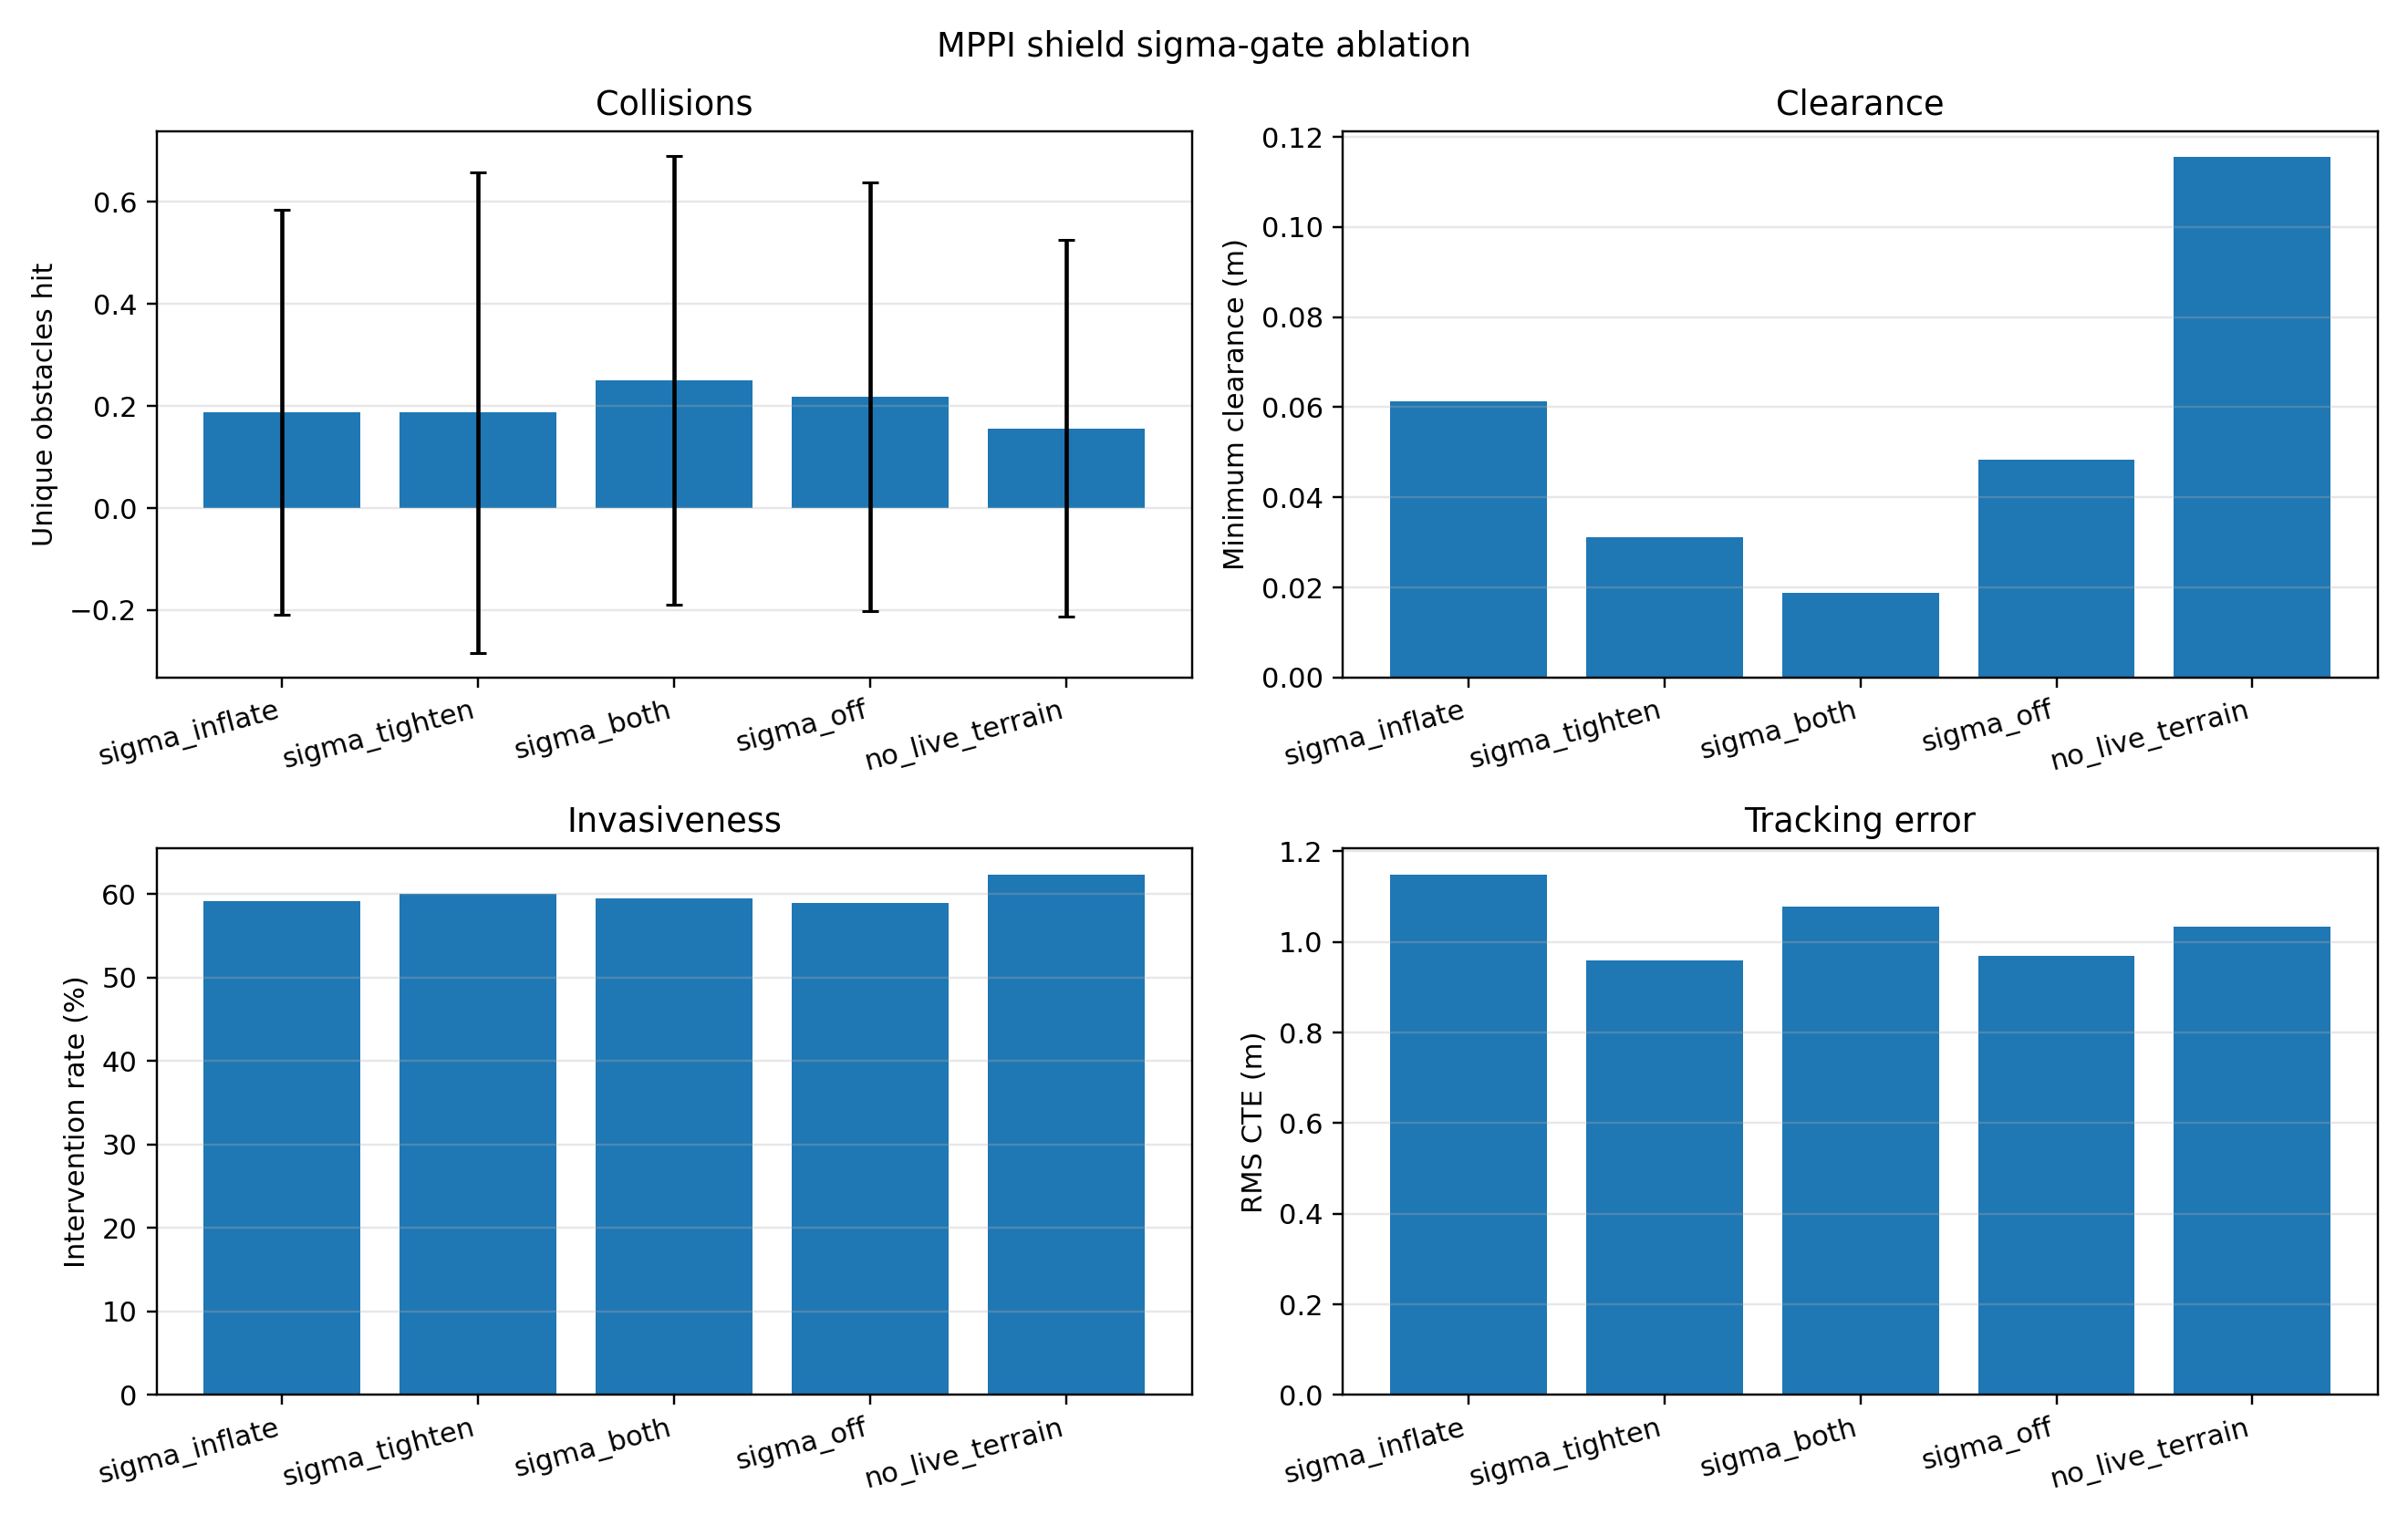
\includegraphics[width=\columnwidth]{sigma_gate_ablation_summary.png}
  \\[2pt]
  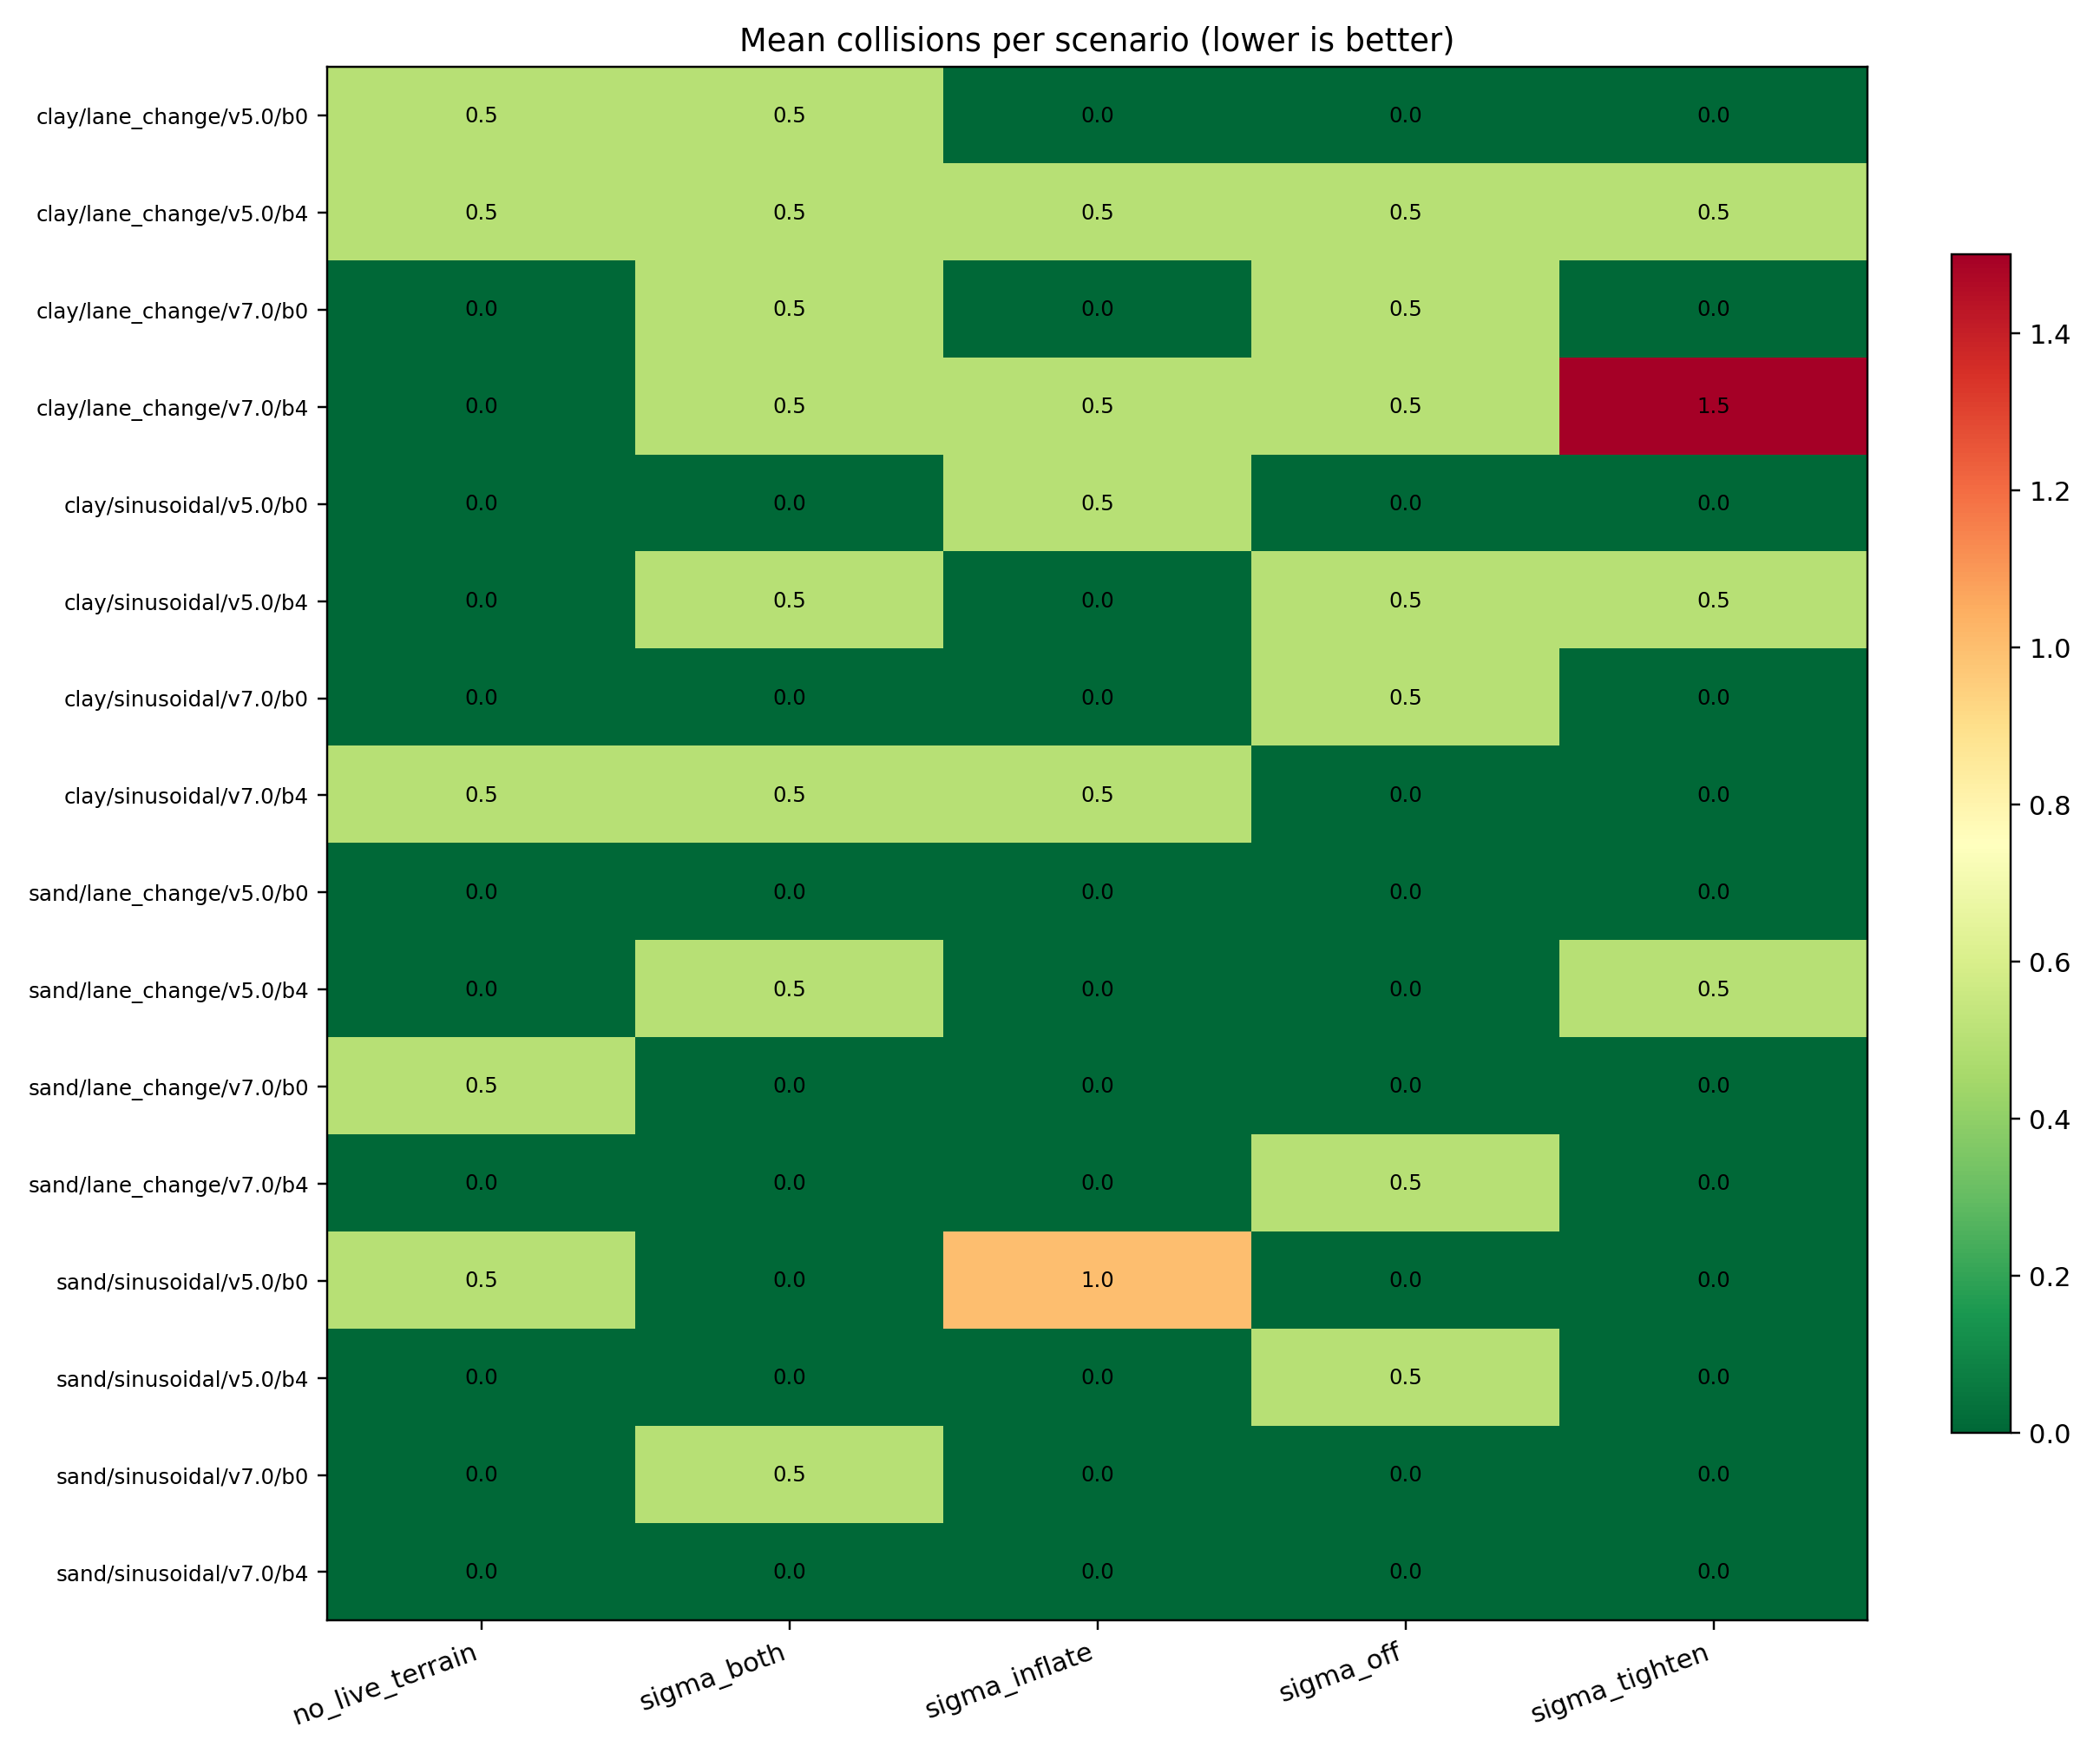
\includegraphics[width=\columnwidth]{sigma_gate_ablation_collision_heatmap.png}
  \caption{$\phi$-uncertainty gate ablation. Top: aggregate
    KPIs. Bottom: per-scenario collisions.}
  \label{fig:phigate}
\end{figure}

%======================================================================
\section{Discussion}
\label{sec:disc}
%======================================================================

The empirical results support the principal architectural choices of
the proposed framework. The neural SCM tire surrogate, evaluated
both with static terrain parameters and with the online estimator
active, attains real-time solve times ($<10\,\mathrm{ms}$) and
reduces RMS crosstrack error by 20--50\,\% relative to the
analytical Pacejka and TMeasy baselines depending on the
configuration. The asymmetric throttle disturbance observer closes
approximately 10\,\% of the soft-soil speed gap with no measurable
tracking cost. The two-layer planner-aware obstacle-avoidance stack
attains zero collisions across the evaluated matrix when paired
with either DOB-CBF or MPPI as the downstream shield, and the MPPI
seed trajectories are shown to be essential rather than auxiliary.
The DOB-CBF filter benefits substantially from re-using the neural
surrogate, and both shields reduce collisions by approximately
85\,\% under the learned N-HiTS 5G traffic profile relative to no
shield.

Two architectural choices are constrained by the same evaluation.
The Model Predictive Contouring Control variant, while attractive
in formulation, attains a worse tracking-vs-speed Pareto point than
the standard reference-tracking NMPC in every configuration tested.
The ensemble-style $\phi$-uncertainty gate on the MPPI shield's
friction cone, evaluated under both the original tighten-cone
formulation and a redesigned inflate-buffer formulation, degrades
collision performance relative to a baseline that ignores live
terrain updates entirely. The final system configuration therefore
omits the $\phi$-gate on the shield and uses the standard NMPC as
the primary planner.

The joint $(n,\phi)$ identification of
Section~\ref{sec:estimator_joint} is established offline on the
rich-excitation Latin-hypercube corpus; the closed-loop estimator
deployed inside the NMPC currently regresses $n$ only, and extending
the live closed-loop path to the joint head is a natural next step.
The human-in-the-loop safety-filter comparison of
Section~\ref{sec:safety_hil} is collected with a Logitech G29
steering rig under symmetric command/camera latency; the autonomous
sweeps reported elsewhere serve as a controlled, repeatable
complement that removes operator variance.

A direction for future work suggested by the negative result of
Section~\ref{sec:phigate_negative} is to design the
estimator-to-shield interface as a low-pass mixture of the live
estimate rather than as a direct overwrite. The hypothesised
failure mode is that the shield's safety calculations were
calibrated against fixed terrain, and an unfiltered live update
during evasive maneuvers introduces fast-time-scale non-stationarity
that the safety cost is not designed to damp. A shield that
attenuated the estimator update during high-cost epochs would test
this hypothesis directly.

%======================================================================
\section*{Reproducibility}

The complete sweep, including every figure and table in this paper,
is reproduced by the following single command in the project's
\texttt{sim} conda environment:
\begin{quote}\small\tt
python paper\_scripts/run\_paper\_suite.py --tier pilot
\end{quote}
The exact result folders backing each figure are catalogued in
\texttt{my\_paper/paper\_figures/README.md}.

%======================================================================
\section*{Acknowledgements}

This work builds on the Chrono::HIL framework~\cite{Zhou23} and
Project Chrono~\cite{Tasora16,Serban19}. The 5G traffic profile is
generated using the public N-HiTS-5G implementation released with
Choi et al.~\cite{Choi23}.

\begin{thebibliography}{9}

\bibitem{Bekker69}
  M.~G.~Bekker, \emph{Introduction to Terrain-Vehicle Systems}.
  Ann Arbor, MI: University of Michigan Press, 1969.

\bibitem{Choi23}
  Y.-H.~Choi \emph{et al.}, ``ML-based 5G traffic generation for
  practical simulations using open datasets,''
  \emph{IEEE Commun.\ Mag.}, vol.~61, pp.~130--136, 2023.

\bibitem{Dallas21}
  J.~Dallas \emph{et al.}, ``Terrain adaptive trajectory planning
  and tracking on deformable terrains,''
  \emph{IEEE Trans.\ Veh.\ Technol.},
  vol.~70, no.~11, pp.~11255--11268, 2021.

\bibitem{Krenn09}
  R.~Krenn and G.~Hirzinger, ``SCM -- a soil contact model for
  multi-body system simulations,'' in
  \emph{Proc.\ Int.\ Soc.\ for Terrain-Vehicle Systems (ISTVS)},
  Bremen, Germany, 2009.

\bibitem{Serban19}
  R.~Serban, M.~Taylor, D.~Negrut, and A.~Tasora,
  ``Chrono::Vehicle: template-based ground vehicle modelling and
  simulation,''
  \emph{Int.\ J.\ Veh.\ Perf.}, vol.~5, no.~1, pp.~18--39, 2019.

\bibitem{Shibly05}
  H.~Shibly, K.~Iagnemma, and S.~Dubowsky, ``An equivalent soil
  mechanics formulation for rigid wheels in deformable terrain,''
  \emph{J.\ Terramech.}, vol.~42, no.~1, pp.~1--13, 2005.

\bibitem{Tasora16}
  A.~Tasora \emph{et al.}, ``Chrono: an open source multi-physics
  dynamics engine,'' in
  \emph{High Performance Computing in Science and Engineering},
  pp.~19--49, Springer, 2016.

\bibitem{Zhang25}
  H.~Zhang \emph{et al.}, ``Shared control of teleoperated vehicles
  with delay-compensated safety filtering,'' in
  \emph{Proc.\ IEEE Conf.\ Control Technol.\ Appl.\ (CCTA)},
  pp.~192--199, 2025.

\bibitem{Zhou23}
  Z.~Zhou \emph{et al.}, ``A Chrono-based framework for large-scale
  traffic simulation with human-in-the-loop,'' 2023.

\end{thebibliography}

\end{document}
